\documentclass[]{article}
\usepackage{graphicx}

%opening
\title{Sentiment Analysis of Tweets and News Media Reporting on Demonetization Issues}

\author{Ambuj Mishra,Sheshan Sheniwal,Sunil Kumar}




\begin{document}

\maketitle
\begin{center}
{\large\bf
Intermediate BTP progress report \\
\vspace{2ex}
Group No   -  24\\
\vspace{2ex}
Supervisor Name - Dr. Pradip Swarnakar}  \\



\end{center}


\section{Thesis Objective}
Compare the sentiments of online tweets and News reports on the topic “Demonetization” and find the relationship between them on the basis of their sentiments.
\section{Gantt chart (Time line of activities - Prepared earlier)}
\includegraphics[scale=0.55]{xy.png}
\includegraphics[scale=0.65]{chart.png}
\section{Short description of activities completed}
{\bf Data Scrapping} : We used data scrapping techniques using Tweetpy library on Python language to extract data from twitter.
\newline
{\bf Data Mining} : We applied data mining techniques to create certain filters to segregate the data extracted in the previous phase on terms of date, user handle.
\newline
{\bf Sentiment Analysis} : We have used Naïve Bayes to find the polarity and subjectivity of the sentences.
\section{Intermediate results }
We have used algorithms for finding the sentiments of the tweets which we have extracted using tweepy and have obtained the polarity of tweets in terms of positive ,negative and neutral and got the fraction in terms of positivity(0.389) , negativity(0.153) and neuterality(0.458).
\begin{center}
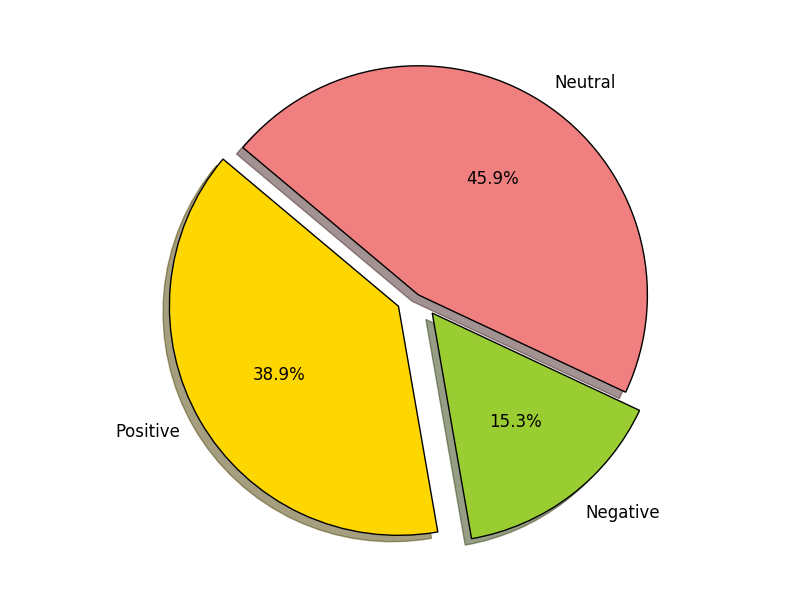
\includegraphics[scale=0.45]{figure1.png}
\end{center}
\section{Future activities }
Now, we intend to begin with the extraction of news reports on “Demonetization” and we will apply algorithms for sentiment analysis to find the polarities of news reports and we will compare the results of both graphically.
\end{document}
